\section{Uniform Spatial Partitioning\label{sec:spatial-partitioning}}

Under \gls{gpu} uniform spatial partitioning the known environment is sub divided into a uniform grid of bins, each given a consecutive identifier (such that in 2 dimensions $i = p^{Y}d^{X}+p^{X}$ where $p$ is the grid position in the corresponding axis and $d$ is the grid's dimensions). Message's locations are then clamped into the known environment bounds, allowing the containing environmental bin to be identified. Messages are sorted and stored in order of their containing bin's identifier.

So that the array of messages can be accessed efficiently, a partition boundary matrix is constructed. This structure provides an index to the start of each bin's messages within the array. Figure \ref{fig:uniform-spatial-partitioning} presents a 2 dimensional example of the data structures used.

\begin{figure*}[!t]
\centering
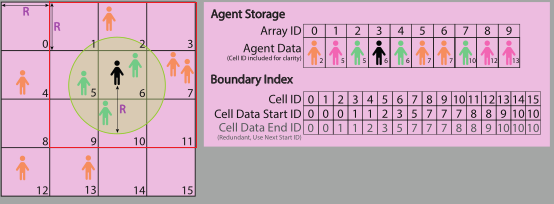
\includegraphics[width=\textwidth]{../resources/usp/placeholder.png}
\caption{\label{fig:uniform-spatial-partitioning}%
\textit{This is a placeholder figure, areas in the left hand grid will be replaced with shading/hashing, and coloured people with symbols. May additionally include the moore neighbourhood arrows.}\newline
Visual representation of an environment and how it's data is stored under \gls{gpu} uniform spatial partitioning.%
The left hand grid represents the environment, where symbols represent messages. The square [hash-sample] and  circular [hash-sample] areas of the environment represent the Moore and radial search neighbourhoods about the search point [symbol-placeholder].%
The tables represent the message storage array (top) and partition boundary matrix respectively.
}
\end{figure*}

Although if the containing bin of a single message changes, the entire data-structure must be reconstructed. The process for constructing both the message array and partition boundary matrix is already highly data-parallel executing in constant time complexity (with respect to the number of messages), if implemented with atomic counting sort\textit{(CITEME? (has Paul published the county sort work), const time scan page 7: https://www.mimuw.edu.pl/~ps209291/kgkp/slides/scan.pdf)}.

In all instances the cost of performing the fixed radius near neighbours search outweighs that of constructing the data-structure. Large neighbourhoods can see the search time take 30x longer than construction, whereas the least demanding configurations (which under utilise the hardware) still perform construction in a third of the time required for search. This is in agreement with the work of Hongyu et al whereby the reconstruction was optimised by sorting from the result of the previous sort\cite{HY*15}. They were able to improve performance in a small \gls{sph} simulation of 8192 particles within a $16^{3}$ grid, however performance was equal to that of their initial unoptimised reconstruction when applied to larger simulations.

Within this paper we have only considered subdivision of the environment such that bin dimensions are equal to the neighbourhood radius. Previously Hoetzlein studied the impact of adjusting bin dimensions, finding the optimal dimension to be $\frac{2}/{3}R$\cite{Hoe14}. However this analysis only considered a fixed density of particles, additionally identifying that it was an optimisation between too many bins and too many messages per bin, the latter which would vary with message density.

To access messages located within the radial neighbourhood of a position, the position's containing environmental bin is identified and all messages stored within the bins of the inclusive Moore neighbourhood are then iterated. Only those with a position inside the radial neighbourhood are forwarded to the model.

In 2 dimensions this means that spatially we are accessing messages with an area 2.86x larger than required (2D neighbourhood area: $\pi R^{2}$, 2D Moore neighbourhood area: $(3R)^{2}$), in 3 dimensions this increases to 6.45x (3D neighbourhood volume: $\frac{4}{3}\pi R^{3}$, 3D Moore neighbourhood volume: $(3R)^{3}$).

\textit{Something about the impact of biased message distribution and GPU execution, which we haven't considered in this paper.}

\textit{Review Goswami space filling (again), see if we can identify where their research differed from our own experience.}
%Goswami et al improved the performance of uniform spatial partitioning neighbour searches during \gls{sph} \cite{GS*10}. Bins within their partitioning are sorted according to a Z-order space-filling curve (also known as a Morton code, this ensures that all particles lying within any power of two aligned block have contiguous Z-indices. This additional locality ensures that more neighbourhoods consist of contiguous blocks of memory, therefore neighbourhood searches are more likely to benefit from contiguous data becoming cached. They utilised a look-up table for Z-indices to ensure efficient construction.

\textit{Describe larger spatial partitioning specific modifications: e.g. neighbourhood grid.}
%#Neighbourhood Grid
%Joselli et al have described a data-structure, neighbourhood grid. This data-structure has been designed to optimise \gls{sph} by assigning each particle to its own bin, rather than the uniformly sized bins found in uniform spatial partitioning \cite{JR*15}. This binning system instead creates an approximate spatial neighbourhood, which has permitted performance improvements of upto 9 times when compared to uniform spatial partitioning methods.
      
%By storing particles to unique bins within a regular grid, neighbourhood searches can be carried out surveying a constant radius of directly adjacent bins. With a radius of 1 cell in 3 dimensions this reduces all neighbourhood searches to checking 26 bins, and in 2 dimensions only 8 bins. This provides constant time queries, rather than queries that increase with the density of particles.

%As particles move, the data-structure must be sorted such that spatial neighbours remain close within the grid. A bi-tonic sort was used in their development and testing, which sorted each dimension in a separate pass, however the focus was on their data-structure and the sorting algorithm used is independent of that. It was clarified that they do not repeat earlier sorts, if the 2nd or 3rd passes also make changes. They found that this would impact the performance, whilst only correcting around a single percentage of particles.